\documentclass[paper=a4paper,jafontsize=9pt,twocolumn,number_oflines=45,line_length=28zw]{myuarticle}

\begin{document}

\title{{\Large\bfseries\gtfamily 価値創造デザイン学類予稿集作成のガイド}}
\author{\\\ 21522000 宮城 花子 \\(指導教員:大和太郎)\\ \\}
\date{}
\maketitle

\section{内容の体裁}
卒業研究成果発表会の予稿の体裁について説明しますが,執筆の際の参考程度と考え,内容の書き方の詳細については各研究室のルールに従って作成するようにしてください.

\subsection{内容サイズ}
内容はA4版とし,余白は,上20mm,下25mm,左右それぞれ20mm程度とってください.本文は2段組とし,段の間隔は2.5字程度としてください.

\subsection{表題部分について}
内容にはタイトルをつけてください.「主題」が14pt,「副題」が11ptで,MSゴシックの太字を基本とします.

\subsection{学籍番号・氏名・指導教員について}
タイトルの下に学籍番号・氏名,さらにその下に指導教員名を記載してください.「学籍番号・氏名」は12pt,「指導教員」は11ptとし,日本語フォントはMS 明朝,英字フォントはTimes New Romanを基本とします.

\subsection{本文について}
見出しは,9ptでMS ゴシックで記載しています.各章・節の番号付けは,各研究室の指示に従ってください.
本文は9ptとし,日本語フォントはMS 明朝,英字フォントはTimes New Romanを基本とします.28字×45行程度の2段組にしてください.
句読点は半角,読点 (,,およびc.) は全角で記載するようにしてください.ただし,参考文献については,読点 は半角で記載してください.
なお,本文内で使われる読点は「,」「.」または「,」「.」のどちらかに統一させてください.

\section{図表}
図表は,必要に応じて適宜配置して結構です.ただし,モノクロ印刷に対応できるようにしてください.

\subsection{キャプション}
図の場合は図の下部に,表の場合はその上部に適切なキャプションを入れるようにして下さい.図表は掲載順に番号を振り,それぞれ「Fig.1 キャプション」,「Tabel.1 キャプション] のように表記してください.図表番号,キャプションともに,9ptでMSゴシックを基本とします.

\subsection{大きさ}
図表の大きさは,各自の判断に任せます.ただし,極端に小さくて見えにくかったり,必要以上に大きなものになったりしないように留意してください.

\subsection{表の例}
\begin{table}[h]
\caption{事業構想学群現学生数}
\label{tab:myu-student-number}
\centering
\begin{tabular}{|p{0.4\columnwidth}|p{0.1\columnwidth}|p{0.1\columnwidth}|p{0.1\columnwidth}|}
  \hline
  学類 & 男 & 女 & 計 \\
  \hline
  事業プランニング & 27  & 49 & 76 \\
  \hline
  事業プランニング & 27  & 49 & 76 \\
  \hline
  事業プランニング & 27  & 49 & 76 \\
  \hline
  事業プランニング & 27  & 49 & 76 \\
  \hline
  \multicolumn{4}{r}{平成30年5月1日現在(単位:人)} \\
\end{tabular}
\end{table}

\subsection{図の例}
\begin{figure}[h]
\centering
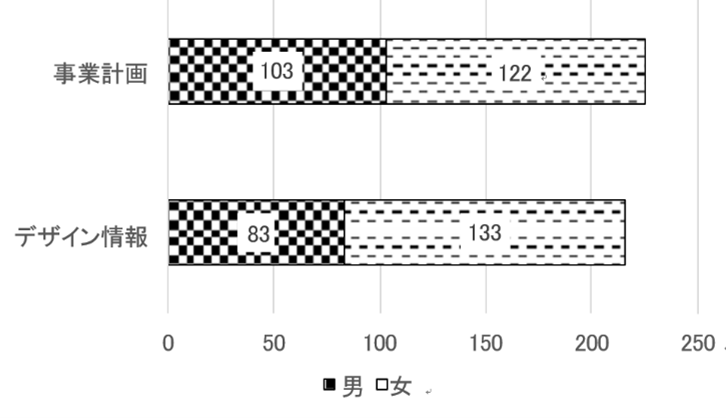
\includegraphics[keepaspectratio, width=0.8\columnwidth]{images/image.png}
\caption[short]{事業構想学部剤学生数}
\label{fig:myu-student-number}
\end{figure}

ちなみに図表のラベル(「図」とか「表」とか)は,myuarticle.clsで設定しているので,「Fig」や「Tab」などにしたい場合は,myuarticle.clsを修正してください.

\section{参考文献の引用の仕方}
文献の引用の仕方は,各研究室の指示に従ってください.
(例)
図書の場合:
【SIST 02 (主に理系)】
著者名. 書名. 出版社, 出版年,  [該ページ数] ,  [シリーズ名] .
【APAスタイル (主に文系)】
著者名(出版年) . 『書名』. 出版社,  [シリーズ名],  [該ページ数] .

雑誌論文の場合:
【SIST 02 (主に理系)】
著者名. 論文名. 誌名. 出版年, 巻号, 号数,  p.始め-終わり.
【APAスタイル (主に文系)】
著者名(出版年) . 「論文名」『誌名』巻号, 号数,  pp.始め-終わり.

ウェブサイトの場合:
【SIST 02 (主に理系)】
著者名. "ページ名". サイト名. 更新日. 入手先URL ,  (参照日) .
【APAスタイル (主に文系)】
著者名(更新日) . "ページ名". サイト名. 入手先URL ,  (参照日).

なおこのガイドでは,バンクーバー方式を使用しています.本文の引用箇所に引用順にA番を振り.文献欄は番号順(引用順)に文献を書きます.

%  ----- 参考文献 -----
\vspace{5pt}
\renewcommand{\refname}{\normalsize 4.  参考文献}
\begin{thebibliography}{9}
% \small % 参考文献の文字サイズを小さくする場合
\bibitem{miyagi2004} 宮城太郎(2004).『〇〇のデザイン』.〇〇文化社.
\bibitem{miyagi2003} 宮城花子(2003). 「〇〇デザイン理論」.『宮城大学学会誌』42巻, 3号, pp.56-70.
\bibitem{yamato2015} 大和太郎(2015). 「事業構想学部学びの事例」.宮城大学, 2015年6月5日, http://www.myu.ac.jp/site/jigyo/jigyomne.html(2023年7月4日参照).
\end{thebibliography}
\bibliographystyle{junsrt}

\end{document}
